% ============================================================
%  poster.tex  —  A0 portrait beamerposter
%  Stochastic Bellhop UQ — Technion SIPL
% ============================================================
\documentclass[final]{beamer}
\mode<presentation>{\usetheme{default}}

\usepackage[orientation=portrait,size=a0,scale=1.4]{beamerposter}
\usepackage{amsmath,amssymb}
\usepackage{graphicx}
\usepackage{booktabs}
\usepackage{multirow}
\usepackage[dvipsnames,table]{xcolor}
\usepackage{multicol}
\usepackage{subcaption}
\usepackage[T1]{fontenc}
\usepackage{lmodern}

\graphicspath{
  {../Methods/MC/}
  {../Methods/Delta/}
  {../Methods/LN3/}
  {../Methods/PCE/}
  {../Methods/Comparison/}
  {../Methods/Methods/MC/}
  {../Methods/Methods/Delta/}
  {../Methods/Methods/LN3/}
  {../Methods/Methods/PCE/}
  {../Methods/Methods/Comparison/}
  {../validation/analytical/figures/}
}

\definecolor{technionblue}{RGB}{0,59,126}
\definecolor{lightblue}{RGB}{220,235,255}
\definecolor{successgreen}{RGB}{0,100,40}
\definecolor{failred}{RGB}{160,30,30}
\definecolor{warnyellow}{RGB}{160,100,0}

\newcommand{\EX}{\mathbb{E}}
\newcommand{\Var}{\mathrm{Var}}
\newcommand{\TL}{\mathrm{TL}}

\setbeamercolor{block title}{fg=white,bg=technionblue}
\setbeamercolor{block body}{fg=black,bg=lightblue!30}
\setbeamercolor{headline}{fg=white,bg=technionblue}

% ============================================================
\begin{document}
% ============================================================

\begin{frame}[t]

%% ── HEADER ──────────────────────────────────────────────────
\begin{beamercolorbox}[wd=\paperwidth,ht=8cm,sep=1cm]{headline}
  {\Huge\bfseries Uncertainty Quantification for Underwater Acoustic\\[4pt]
   Transmission Loss: Delta, PCE, LN3, and Monte Carlo}\\[8pt]
  {\Large O.~Dig \quad $\cdot$ \quad Signal and Image Processing Laboratory (SIPL)
          \quad $\cdot$ \quad Technion --- Israel Institute of Technology}\\[4pt]
  {\large 2026}
\end{beamercolorbox}

\vspace{0.5cm}

%% ── THREE COLUMNS ───────────────────────────────────────────
\begin{columns}[T,totalwidth=\paperwidth]

%% ══════════════════════════════════════
%% COLUMN 1 — Motivation & Methods
%% ══════════════════════════════════════
\begin{column}{0.32\paperwidth}

\begin{block}{Motivation}
Sonar mission planning requires probabilistic Transmission Loss (TL) maps
rather than single-value Bellhop predictions.
Environmental inputs (frequency, source depth $z_S$, SVP) are uncertain,
and their effect on the TL field must be quantified.

\vspace{0.5em}
\textbf{Uncertain parameters:}
\begin{itemize}\small
  \item $f \sim \mathcal{N}(\mu_f,\, \sigma_f^2)$, $\sigma_f = p\mu_f/200$
  \item $z_S \sim \mathcal{N}(\mu_z,\, \sigma_z^2)$, $\sigma_z = p\mu_z/200$
  \item $\Delta T \sim \mathcal{N}(0,\, \sigma_s^2)$ (coupled MLD shift)
\end{itemize}
Uncertainty levels: $p \in \{1\%,\, 5\%,\, 10\%\}$\\[0.5em]
5 propagation scenarios, $N{=}1000$ Bellhop runs each.
\end{block}

\vspace{0.5em}
\begin{block}{Method 1: Bellhop-FD Delta (FOSM)}
First-order linearisation (same as FOSM/GUM):
\begin{equation}
  \Var_1[\TL] \approx \sum_i J_i^2 \sigma_i^2, \quad
  J_i = \frac{\partial\TL}{\partial\theta_i}\bigg|_{\boldsymbol\theta_0}
\end{equation}
Jacobian via \textbf{Bellhop Finite-Difference} (Bellhop-FD): 2 extra runs per parameter.\\
2nd-order correction: $\Var_2 \approx \Var_1 + \tfrac{1}{2}\sum_i H_{ii}^2\sigma_i^4$
\end{block}

\vspace{0.5em}
\begin{block}{Method 2: PCE with LOO-CV Order Selection}
\begin{equation}
  \TL(\theta) \approx \sum_{n=0}^K c_n \Phi_n(\xi), \quad \xi = \frac{\theta - \theta_0}{\sigma}
\end{equation}
QR regression on $N{=}50$ cached samples — \textit{zero new Bellhop runs}.\\
Analytic LOO-CV order selection: $K^* = \arg\min_K\,\overline{\mathrm{LOO}}(K)$,
computed from hat-matrix diagonal $h_{ii}$ of the QR factor.
\end{block}

\vspace{0.5em}
\begin{block}{Method 3: LN3 Distribution Fit}
Physical motivation: mode-sum CLT $\Rightarrow$ $|p| \sim$ Rayleigh $\Rightarrow$ $\TL \sim$ LN3.
\begin{equation}
  X - \gamma \sim \mathrm{LN2}, \quad \gamma = 0.95\min(\mathrm{samples})
\end{equation}
Method of moments (MLE inapplicable: LHS samples are not i.i.d.).\\
\textbf{Delta--LN3 hybrid:} matches LN3 moments to analytically computed
$\EX[\TL]$, $\Var[\TL]$ --- no MC needed for $P_\mathrm{fail}$ estimation.
\end{block}

\vspace{0.5em}
\begin{block}{Method 4: Monte Carlo Ground Truth}
$N{=}1000$ Bellhop samples per scenario/distribution (LHS + IID + SVP).\\
Importance sampling reweights Normal\,10\% ensemble for 5\% and 1\%.\\
$N{=}300$ sufficient for $<5\%$ relative RMSE of $\Var[\TL]$.

\begin{center}
  
\includegraphics[width=0.82\linewidth]{deep_water/Normal_5pct/figures/svp_ensemble.png}
  \captionof{figure}{\small SVP ensemble, deep water, Normal\,5\%, $N=1000$.}
\end{center}
\end{block}

\vspace{0.5em}
\begin{block}{Pipeline Architecture}
\begin{center}
  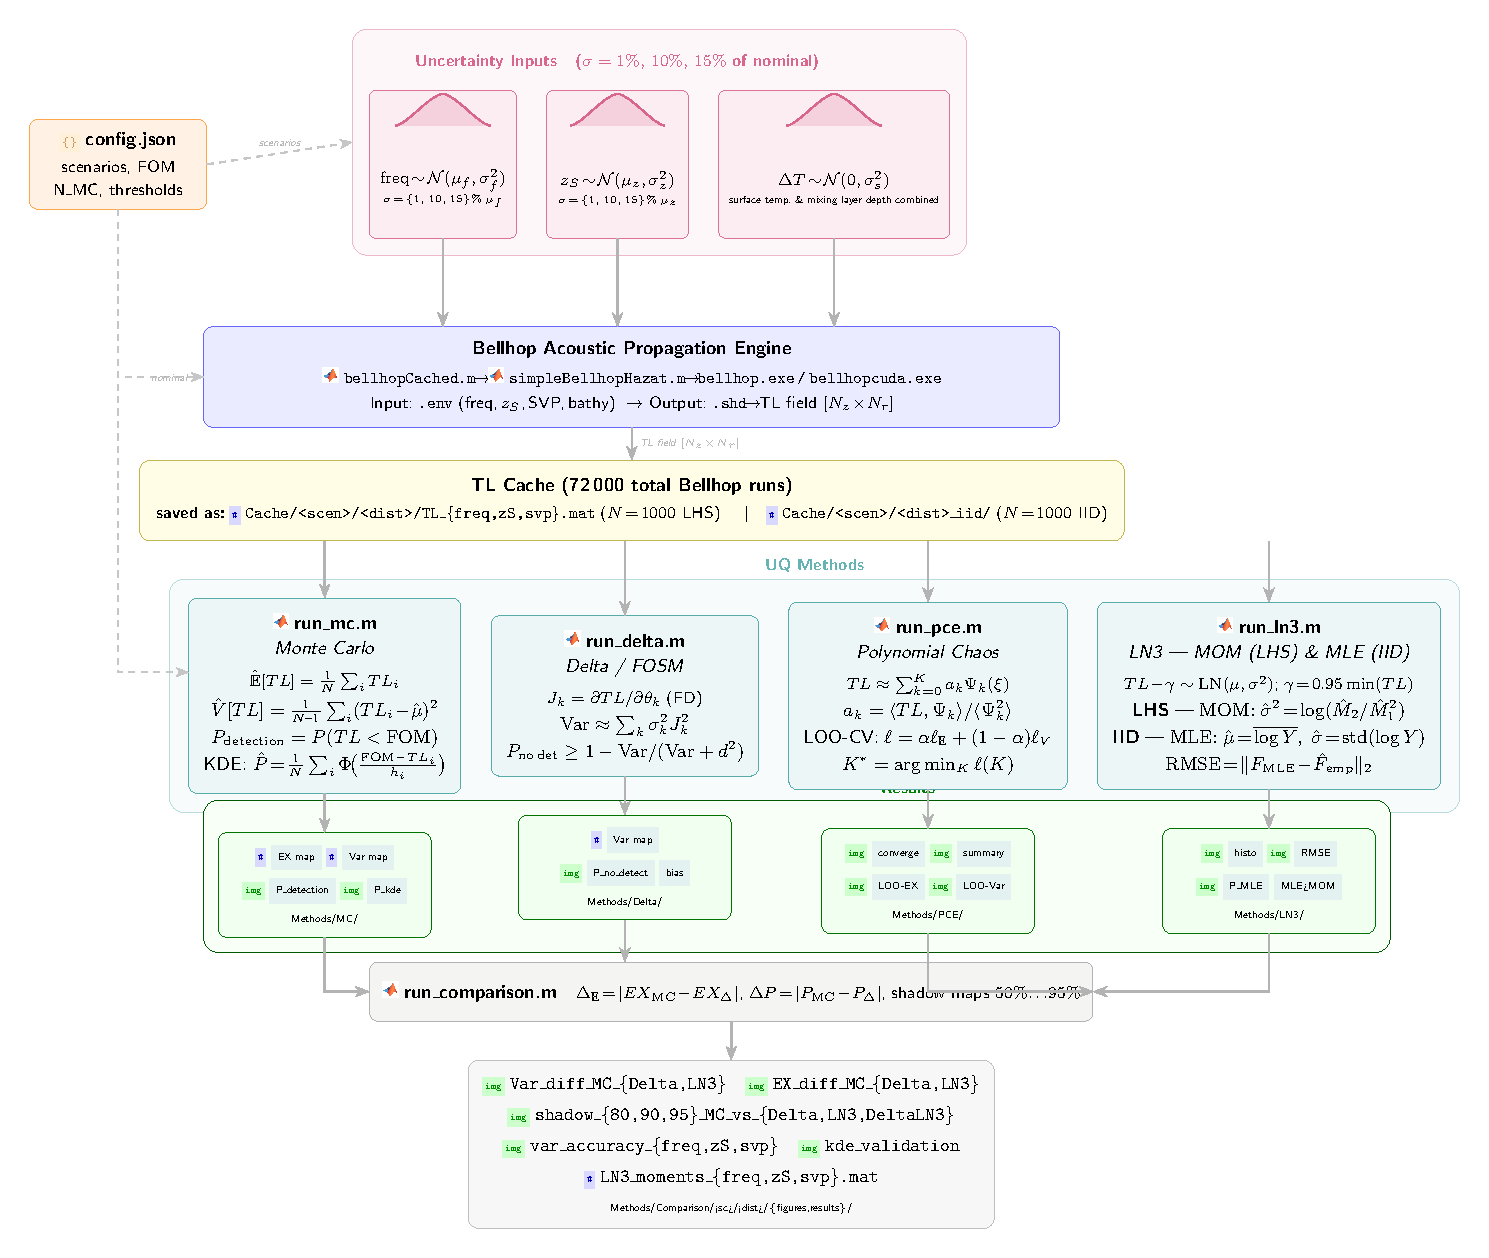
\includegraphics[width=0.85\linewidth]{../docs/block_diagram.pdf}
\end{center}
\end{block}

\end{column}

%% ══════════════════════════════════════
%% COLUMN 2 — Delta & Validation Results
%% ══════════════════════════════════════
\begin{column}{0.34\paperwidth}

\begin{block}{Analytical Validation of Bellhop-FD Jacobian}
Compared Bellhop-FD Jacobian $\partial\TL/\partial z_S$ to closed-form waveguide solution.
$L_1 < 5\%$ at all uncertainty levels $\Rightarrow$ Bellhop-FD is accurate.

\begin{center}
  
\includegraphics[width=0.82\linewidth]{delta_validation_Normal_5pct.png}
  \captionof{figure}{\small Bellhop-FD vs.\ analytical Jacobian, Normal\,5\% $z_S$ uncertainty.
             Four panels: TL\,(Bellhop), TL\,(analytical), $\partial\TL/\partial z_S$\,(Bellhop-FD),
             $\partial\TL/\partial z_S$\,(analytical). Close agreement validates the method.}
\end{center}
\end{block}

\vspace{0.5em}
\begin{block}{Delta Method: Where It Works and Where It Fails}

\begin{center}
  \begin{subfigure}{0.47\linewidth}
    
\includegraphics[width=\linewidth]{baseline/Uniform_1pct/figures/shadow_70_MC_vs_Delta.png}
    \caption{\small Uniform\,1\%: Delta agrees with MC}
  \end{subfigure}
  \hfill
  \begin{subfigure}{0.47\linewidth}
    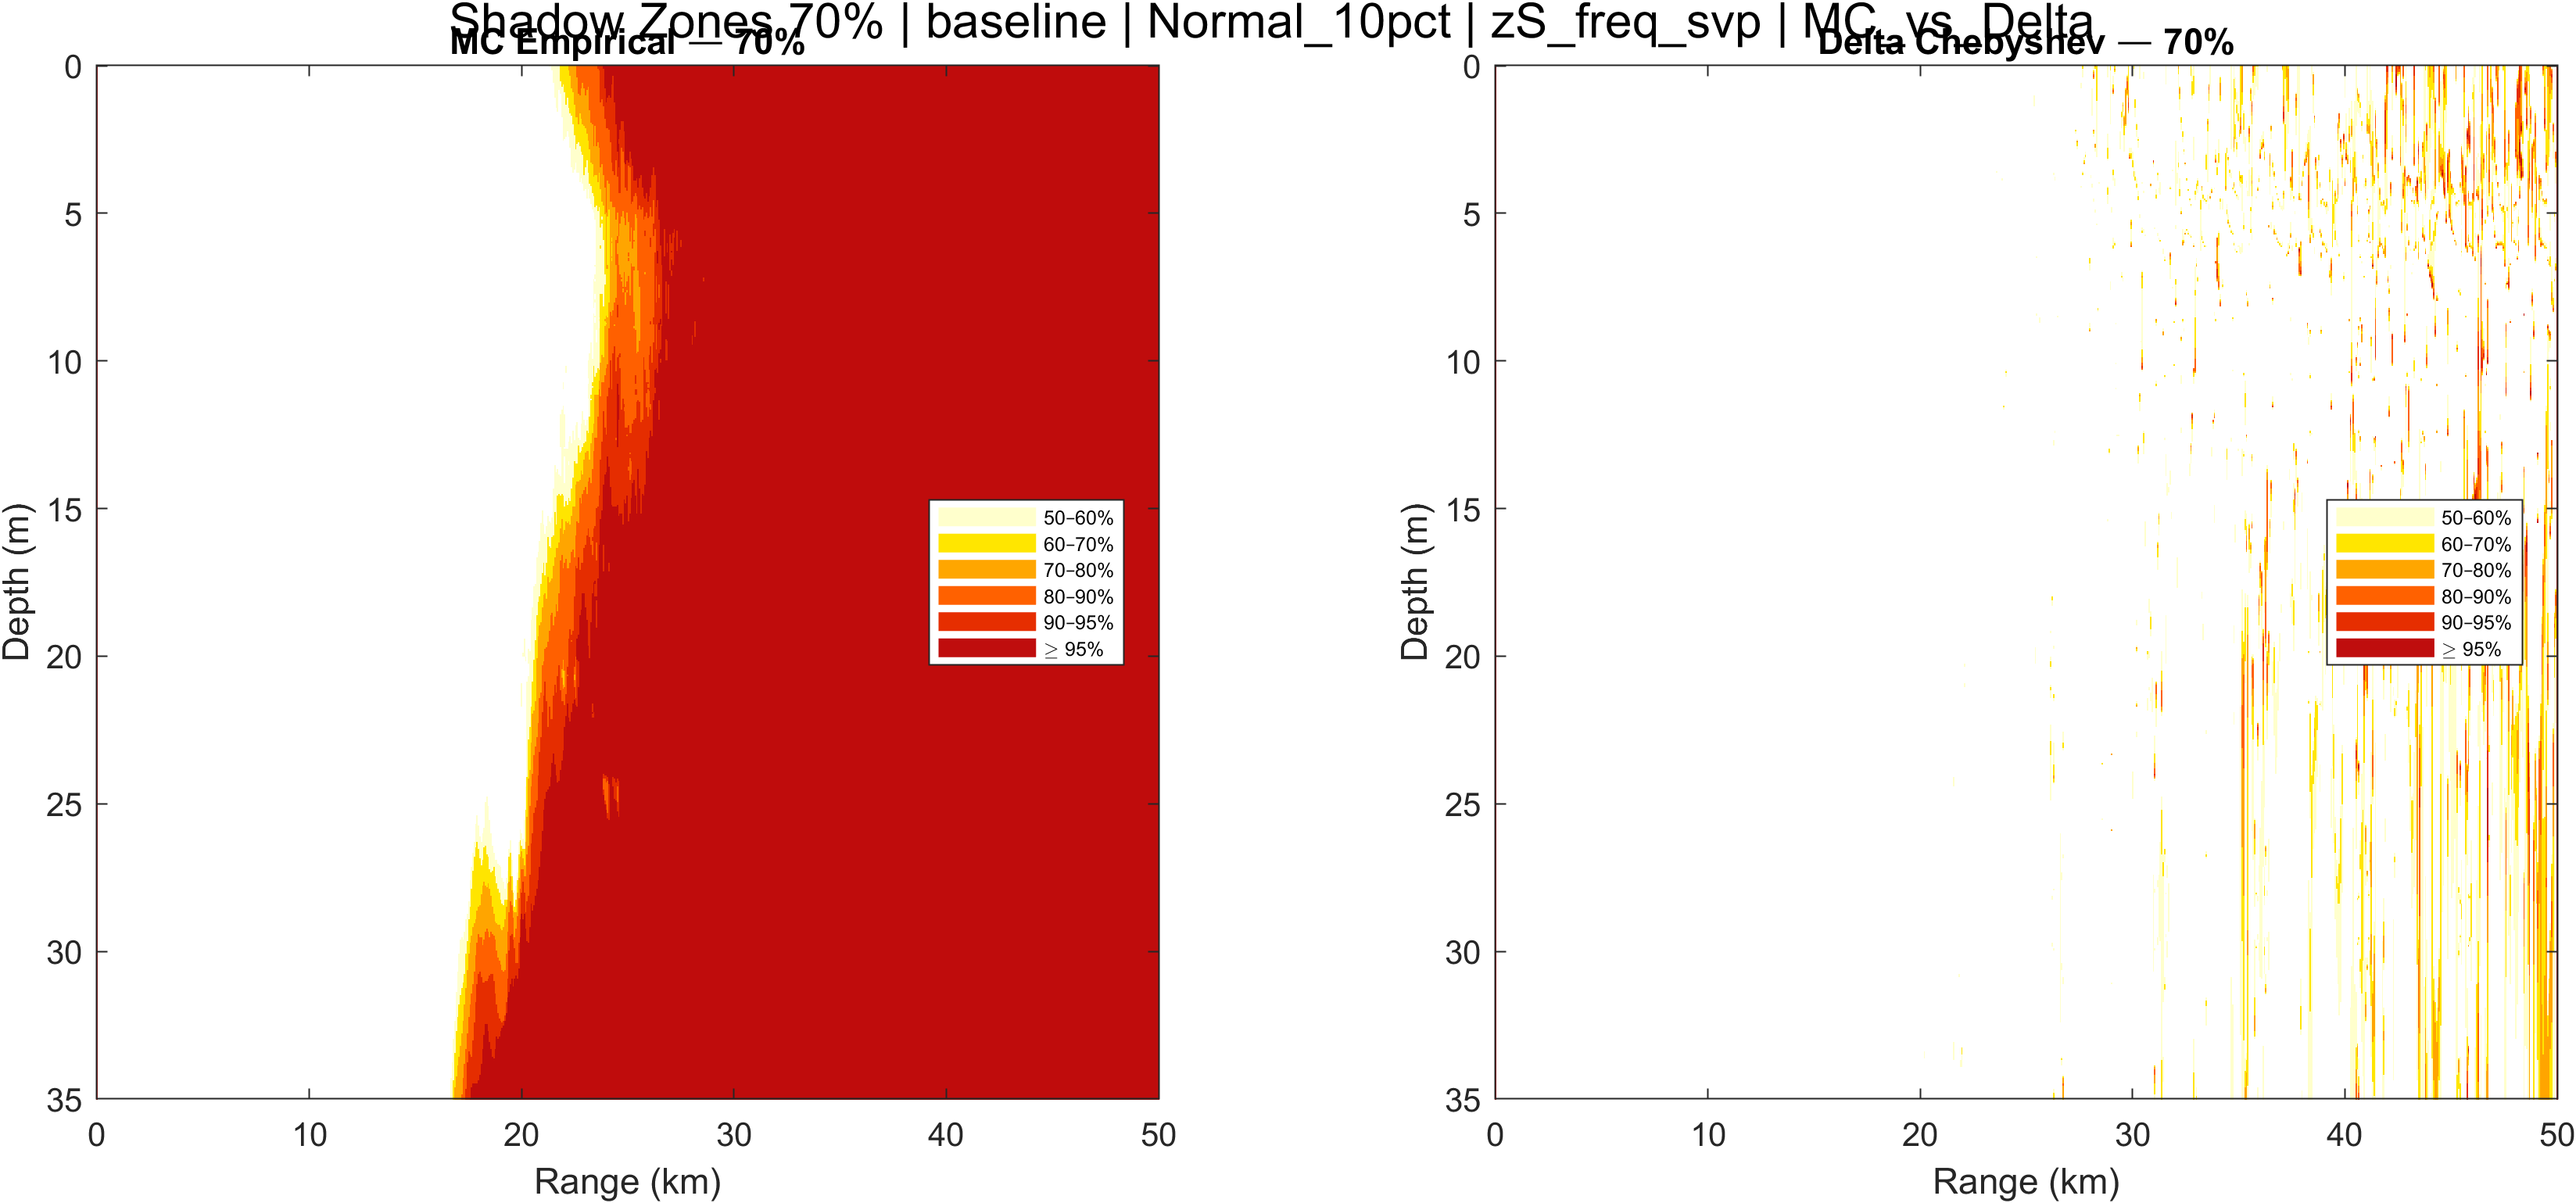
\includegraphics[width=\linewidth]{baseline/Normal_10pct/figures/shadow_70_MC_vs_Delta.png}
    \caption{\small Normal\,10\%: Delta fails}
  \end{subfigure}
\end{center}

\vspace{0.5em}
\begin{center}
  \begin{subfigure}{0.47\linewidth}
    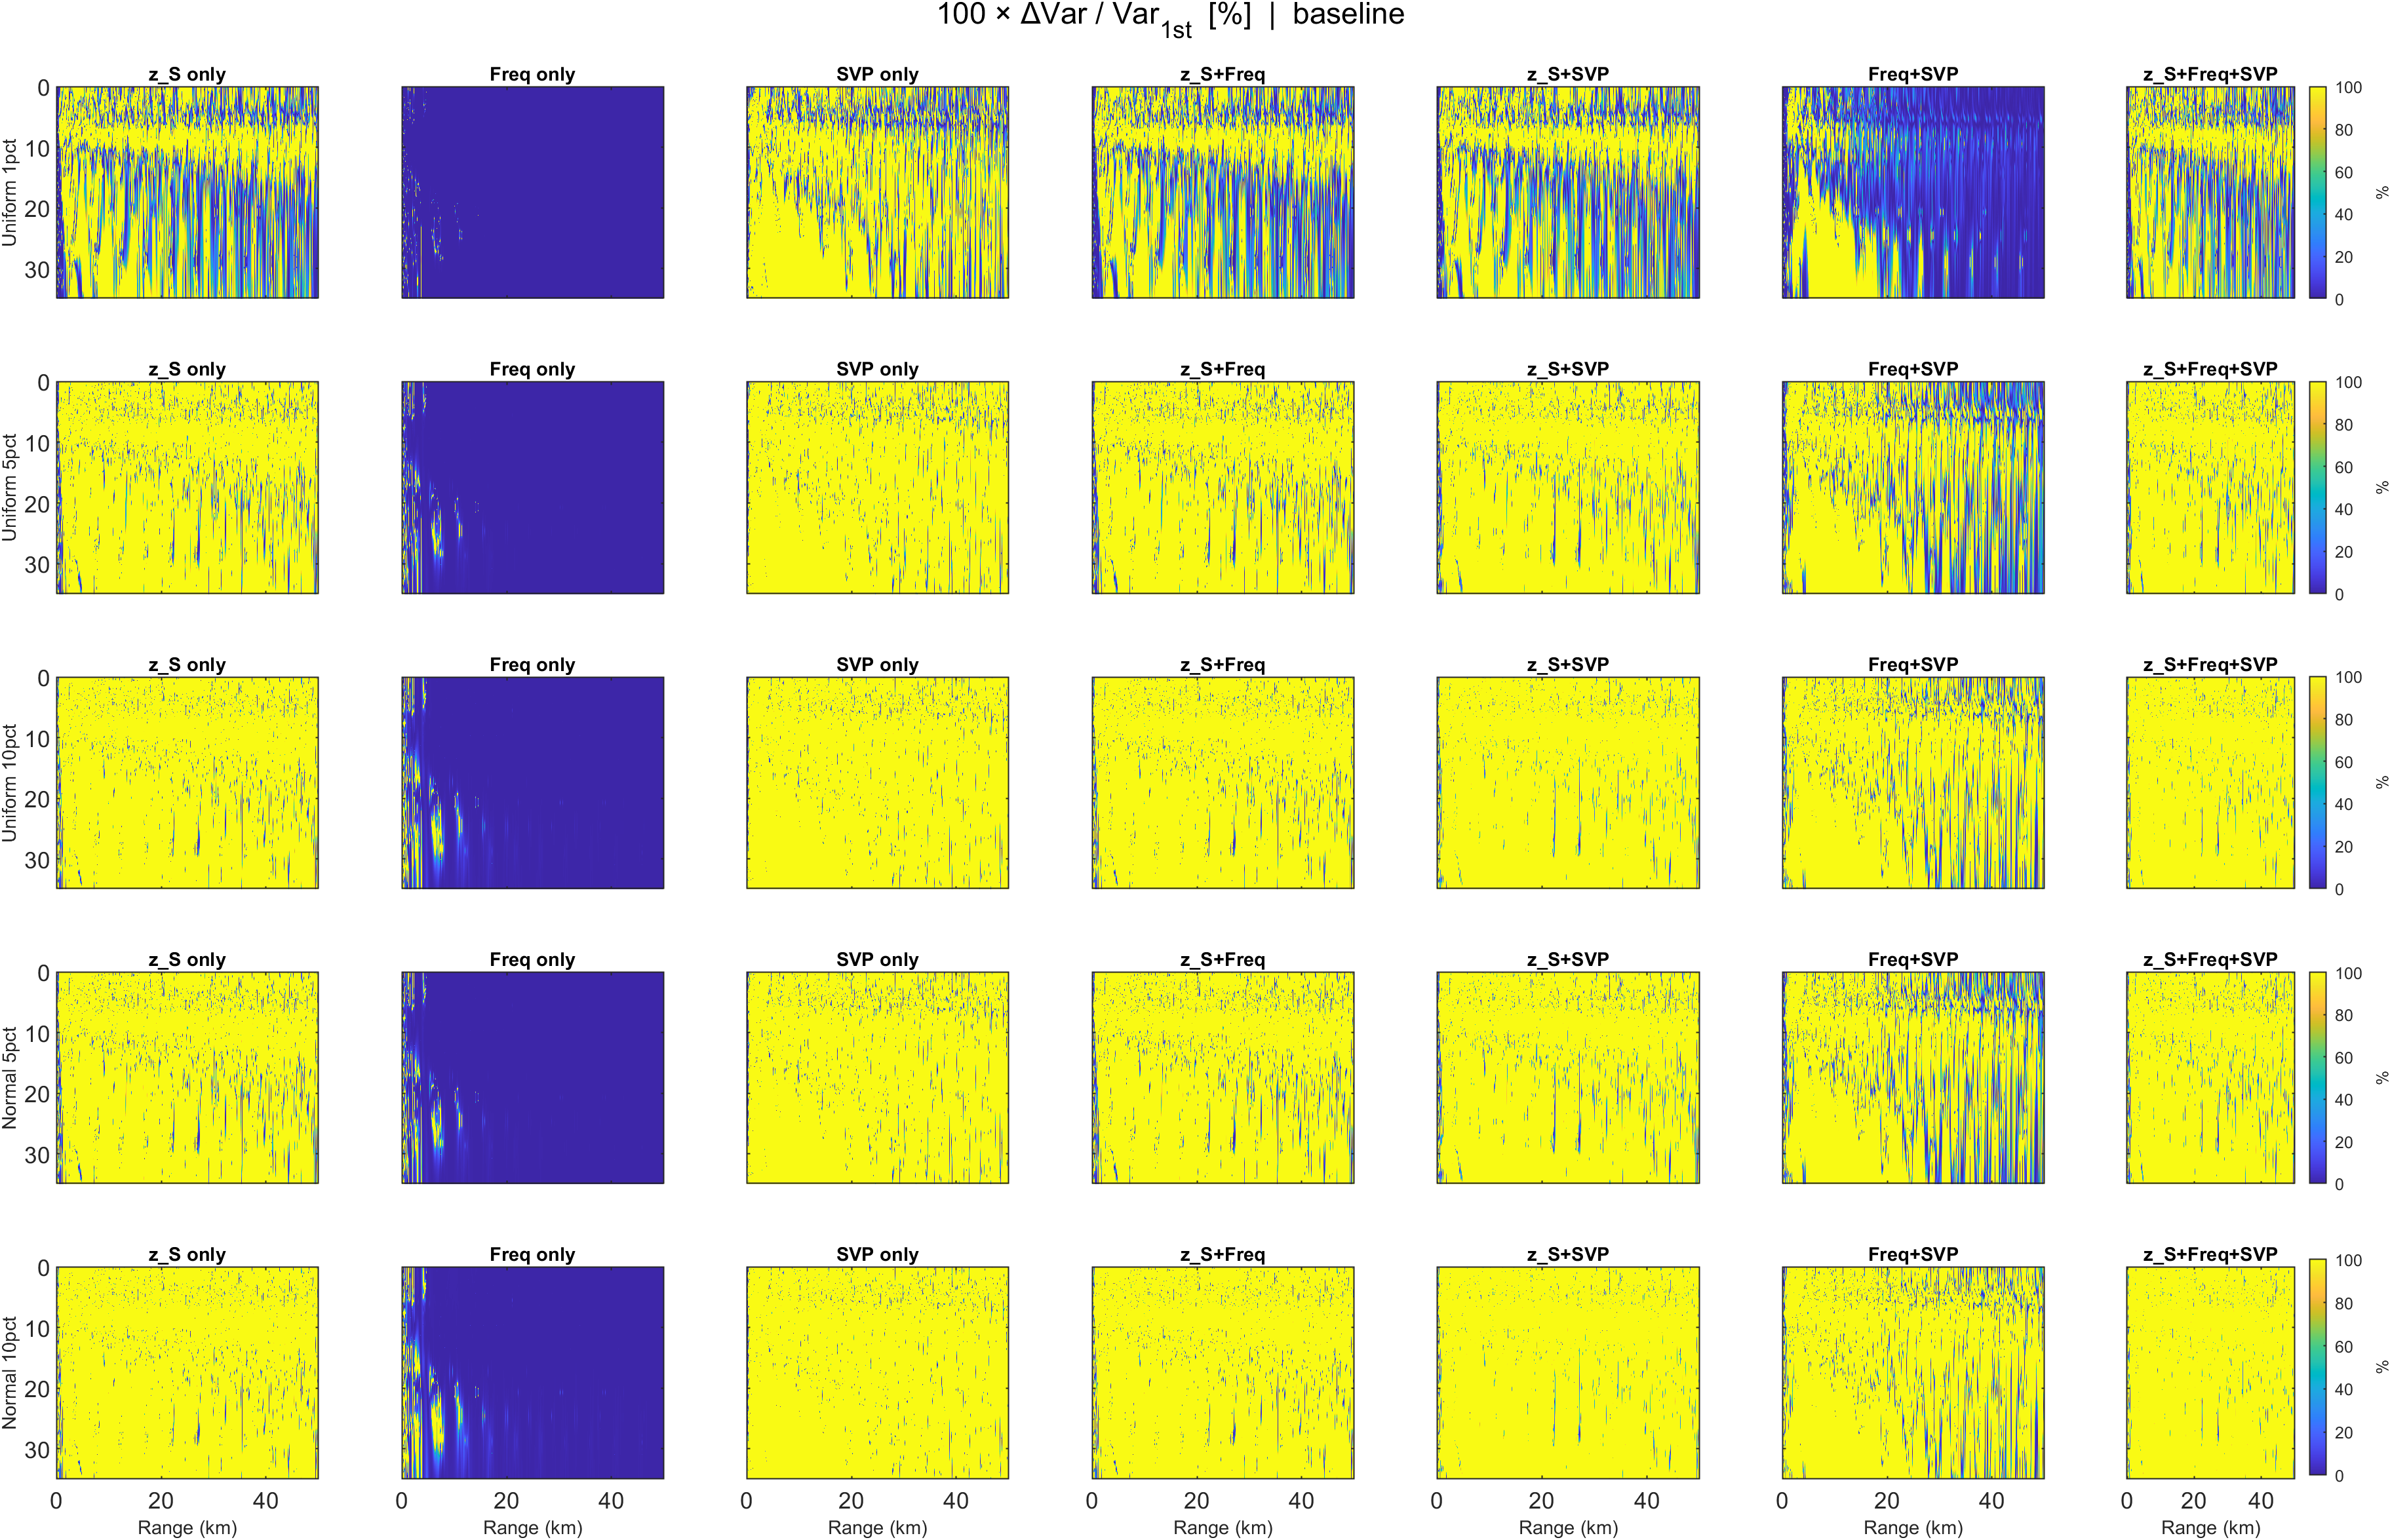
\includegraphics[width=\linewidth]{baseline/delta_order_diff_relative.png}
    \caption{\small Baseline: 2nd/1st order ratio}
  \end{subfigure}
  \hfill
  \begin{subfigure}{0.47\linewidth}
    
\includegraphics[width=\linewidth]{downslope/delta_order_diff_relative.png}
    \caption{\small Downslope: 2nd/1st ratio — red everywhere}
  \end{subfigure}
\end{center}

\renewcommand{\arraystretch}{1.2}
\begin{center}
\begin{tabular}{lcc}\small
  \toprule
  Scenario & Normal\,5\% & Normal\,10\% \\
  \midrule
  Baseline (flat) & 96.6\% & 99.1\% \\
  Deep water      & 97.0\% & 99.2\% \\
  Upslope         & 97.5\% & 99.4\% \\
  Downslope       & 96.1\% & 99.0\% \\
  \bottomrule
\end{tabular}
\end{center}
\vspace{0.3em}
{\small Mean 2nd-order Hessian correction. Values $>$50\% indicate
1st-order insufficient. $>$96\% means even 2nd order has not converged.}
\end{block}

\vspace{0.5em}
\begin{block}{LN3 Distribution Fit}
{\small KS statistic $D_\mathrm{KS} = \sup_x|F_\mathrm{emp} - F_\mathrm{LN3}|$.
$D_\mathrm{crit} \approx 0.043$ at $N{=}1000$.}

\begin{center}
\begin{tabular}{lccc}\small
  \toprule
  Scenario & 1\% & 5\% & 10\% \\
  \midrule
  Deep water    & 0.076 & 0.114 & 0.104 \\
  Shallow water & 0.029 & 0.124 & 0.135 \\
  Upslope       & 0.059 & 0.126 & 0.167 \\
  Downslope     & 0.129 & 0.134 & 0.122 \\
  \bottomrule
\end{tabular}
\end{center}
\vspace{0.3em}
\textbf{All formally rejected} at $N{=}1000$, but $D_\mathrm{KS} \in [0.076, 0.167]$
is a \textit{close geometric fit} — rejection is a large-$N$ artefact, not an engineering failure.
\end{block}

\end{column}

%% ══════════════════════════════════════
%% COLUMN 3 — PCE & Operational Results
%% ══════════════════════════════════════
\begin{column}{0.32\paperwidth}

\begin{block}{PCE Convergence}
\begin{center}
  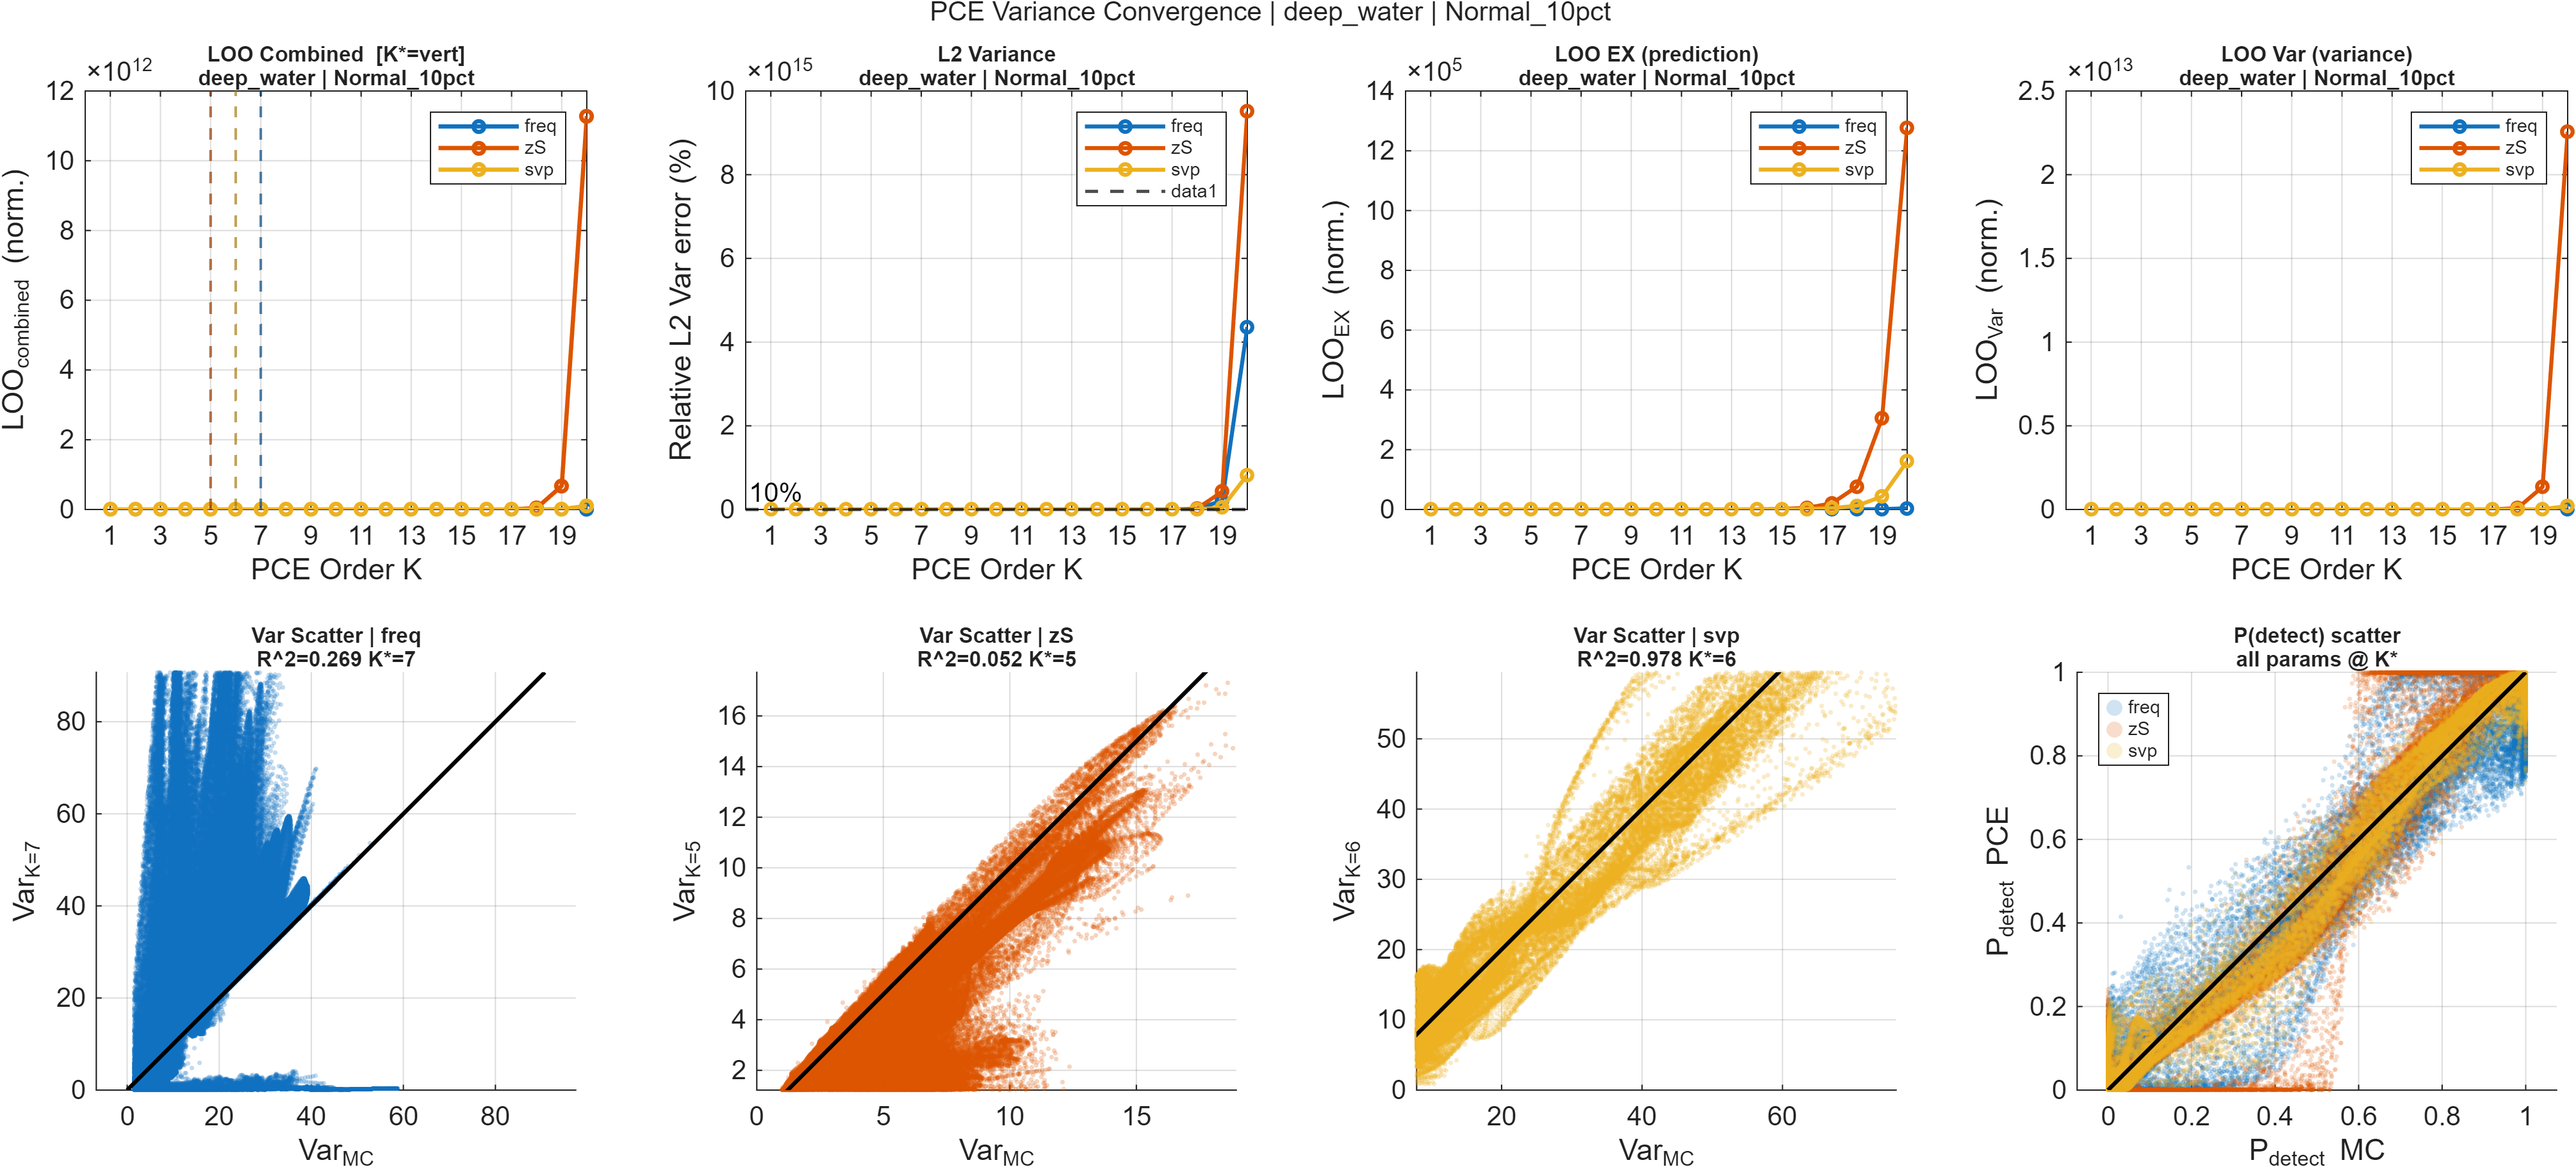
\includegraphics[width=0.95\linewidth]{deep_water/Normal_10pct/figures/pce_convergence_deep_water_Normal_10pct.png}
  \captionof{figure}{\small PCE $L_1$ error vs.\ order $K$, deep water, Normal\,10\%.
             Freq (blue) converges at $K^*{=}5$; SVP (green) at $K^*{=}4$;
             $z_S$ (red) \textbf{never converges} at any $K \leq 20$.}
\end{center}
\end{block}

\vspace{0.5em}
\begin{block}{\colorbox{failred!15}{\textcolor{failred}{NEW FINDING:} $z_S$ Resists PCE Convergence}}
\begin{center}
  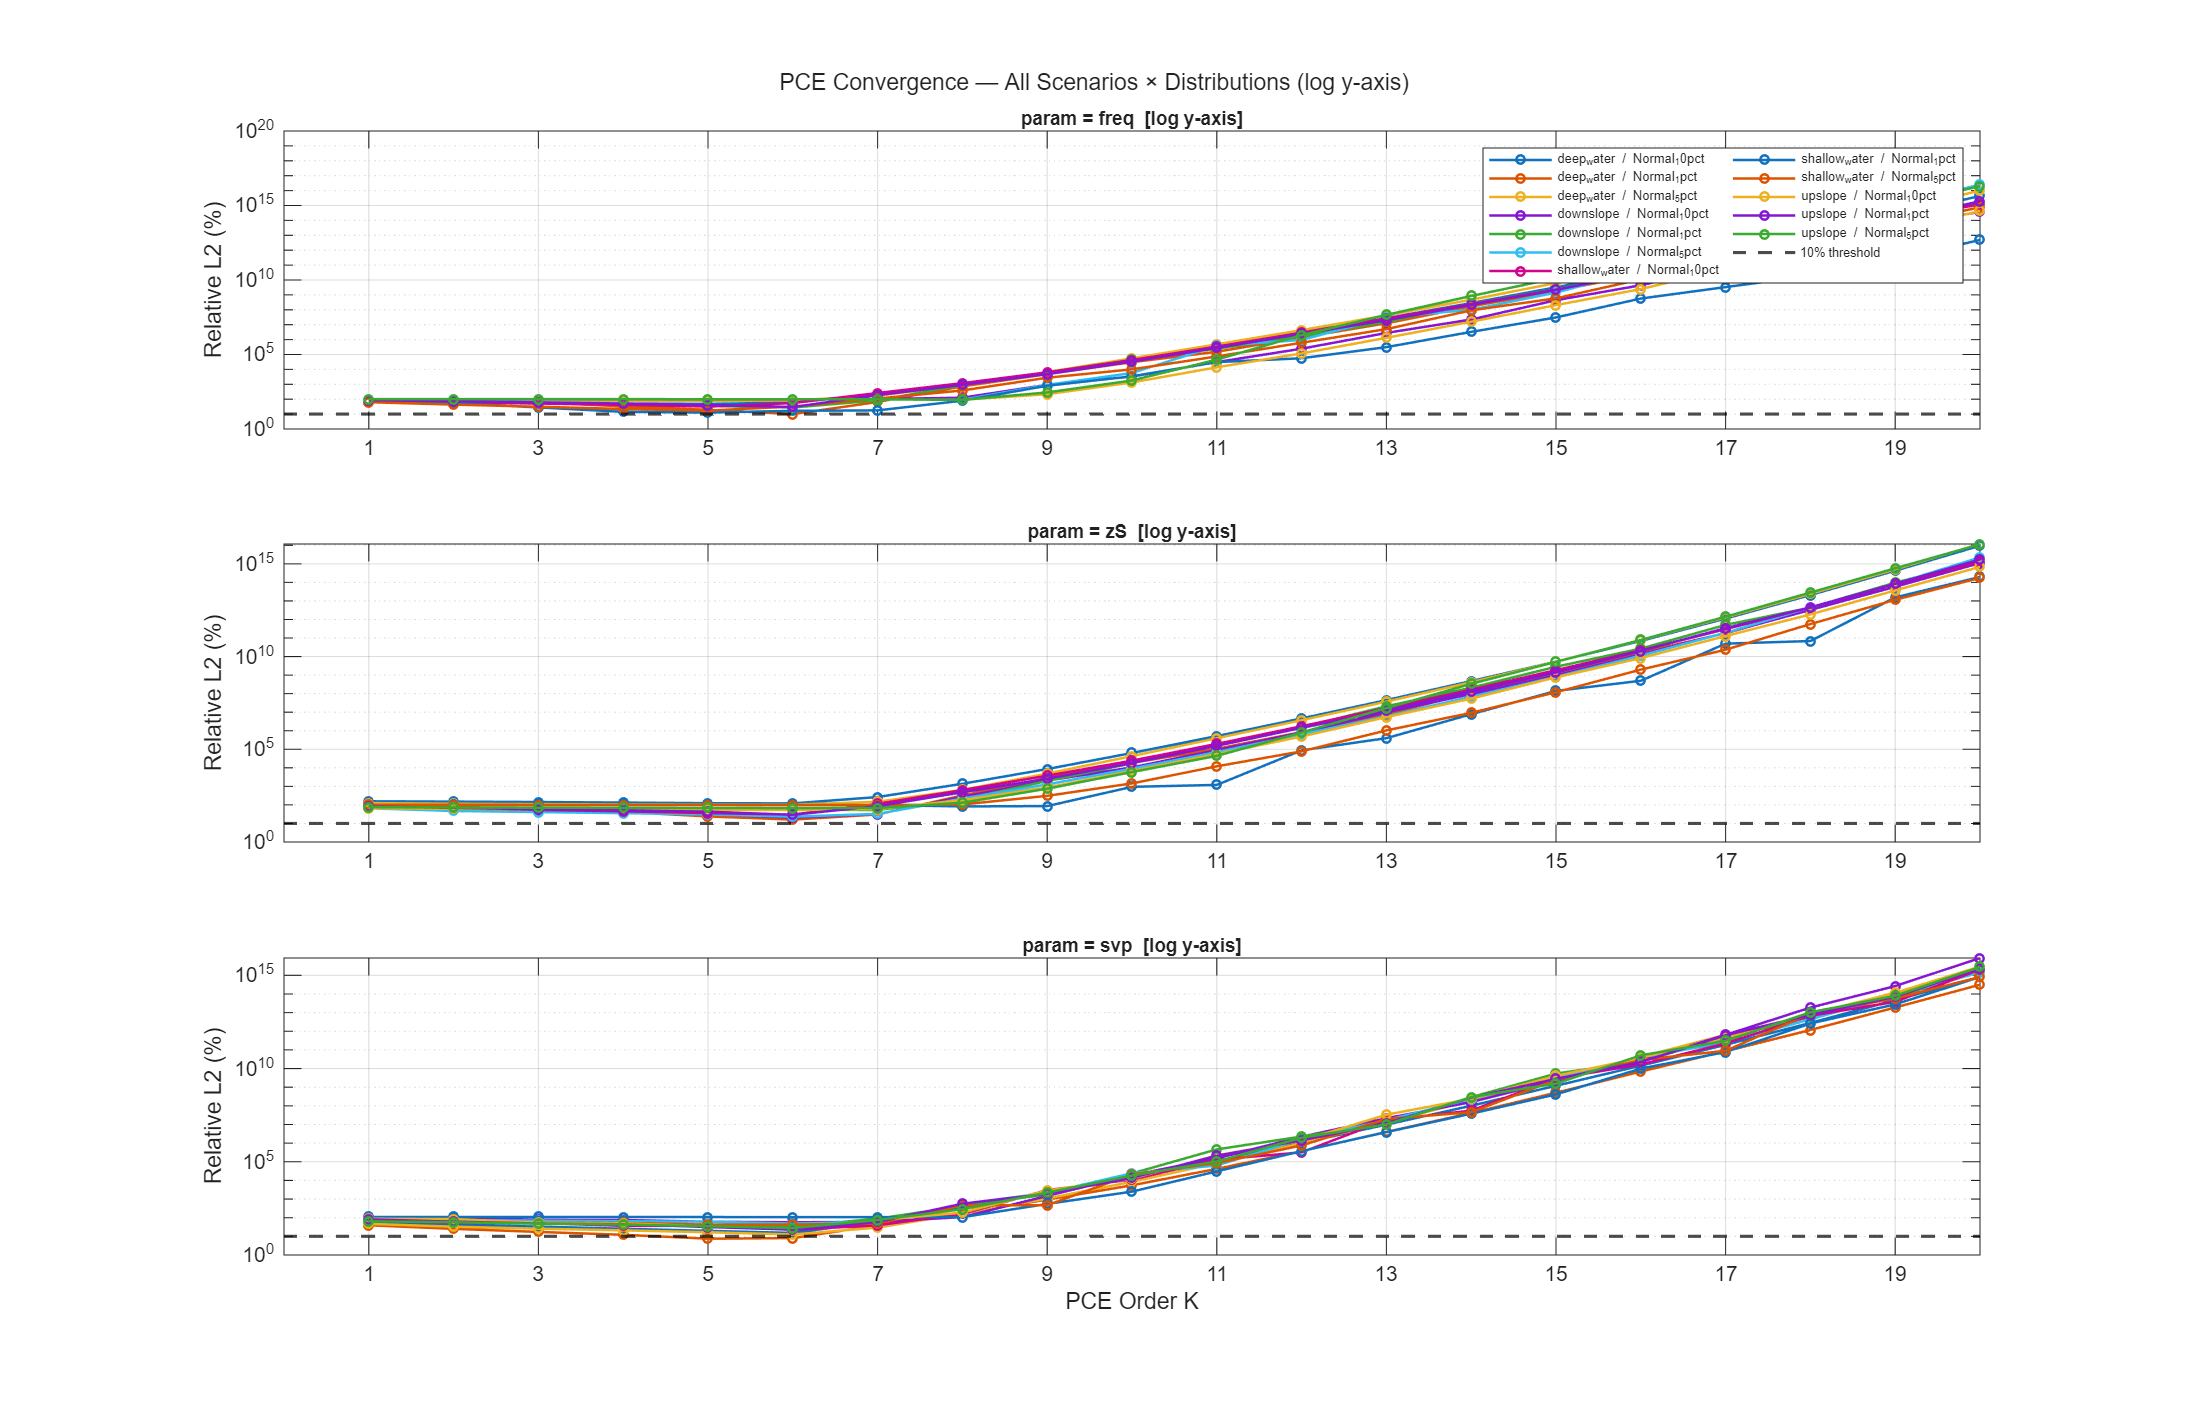
\includegraphics[width=0.92\linewidth]{pce_summary_all.png}
  \captionof{figure}{\small PCE $L_1$ across all 12 scenario/distribution pairs.
             \textbf{$z_S$ curves (red/orange) never reach the 10\% threshold} for Normal $\geq$5\%
             in \textit{any} scenario. Physical cause: source-depth shifts near the
             SOFAR axis cause strongly nonlinear jumps in modal excitation $\psi_m(z_S)$.}
\end{center}

\begin{center}
\renewcommand{\arraystretch}{1.1}
\begin{tabular}{llccc}\small
  \toprule
  Scenario & Dist. & freq & $z_S$ & SVP \\
  \midrule
  Deep water & 1\% & 3 & 3 & 3 \\
  Deep water & 5\% & 6 & \textbf{$>$10} & 3 \\
  Deep water & 10\% & 5 & \textbf{$>$10} & 4 \\
  \midrule
  Downslope  & 5\%  & \textbf{$>$10} & 8 & \textbf{$>$10} \\
  Downslope  & 10\% & \textbf{$>$10} & \textbf{$>$10} & \textbf{$>$10} \\
  \bottomrule
\end{tabular}
\end{center}
{\small $K^*$ = minimum PCE order achieving $L_1 < 10\%$ ($>$10: no convergence).}
\end{block}

\vspace{0.5em}
\begin{block}{Operational Metric: $P_\mathrm{fail}$ Maps}
\begin{center}
  \begin{subfigure}{0.31\linewidth}
    
\includegraphics[width=\linewidth]{deep_water/Normal_5pct/figures/detect_empirical_freq.png}
    \caption{\small freq}
  \end{subfigure}
  \hfill
  \begin{subfigure}{0.31\linewidth}
    
\includegraphics[width=\linewidth]{deep_water/Normal_5pct/figures/detect_empirical_zS.png}
    \caption{\small $z_S$}
  \end{subfigure}
  \hfill
  \begin{subfigure}{0.31\linewidth}
    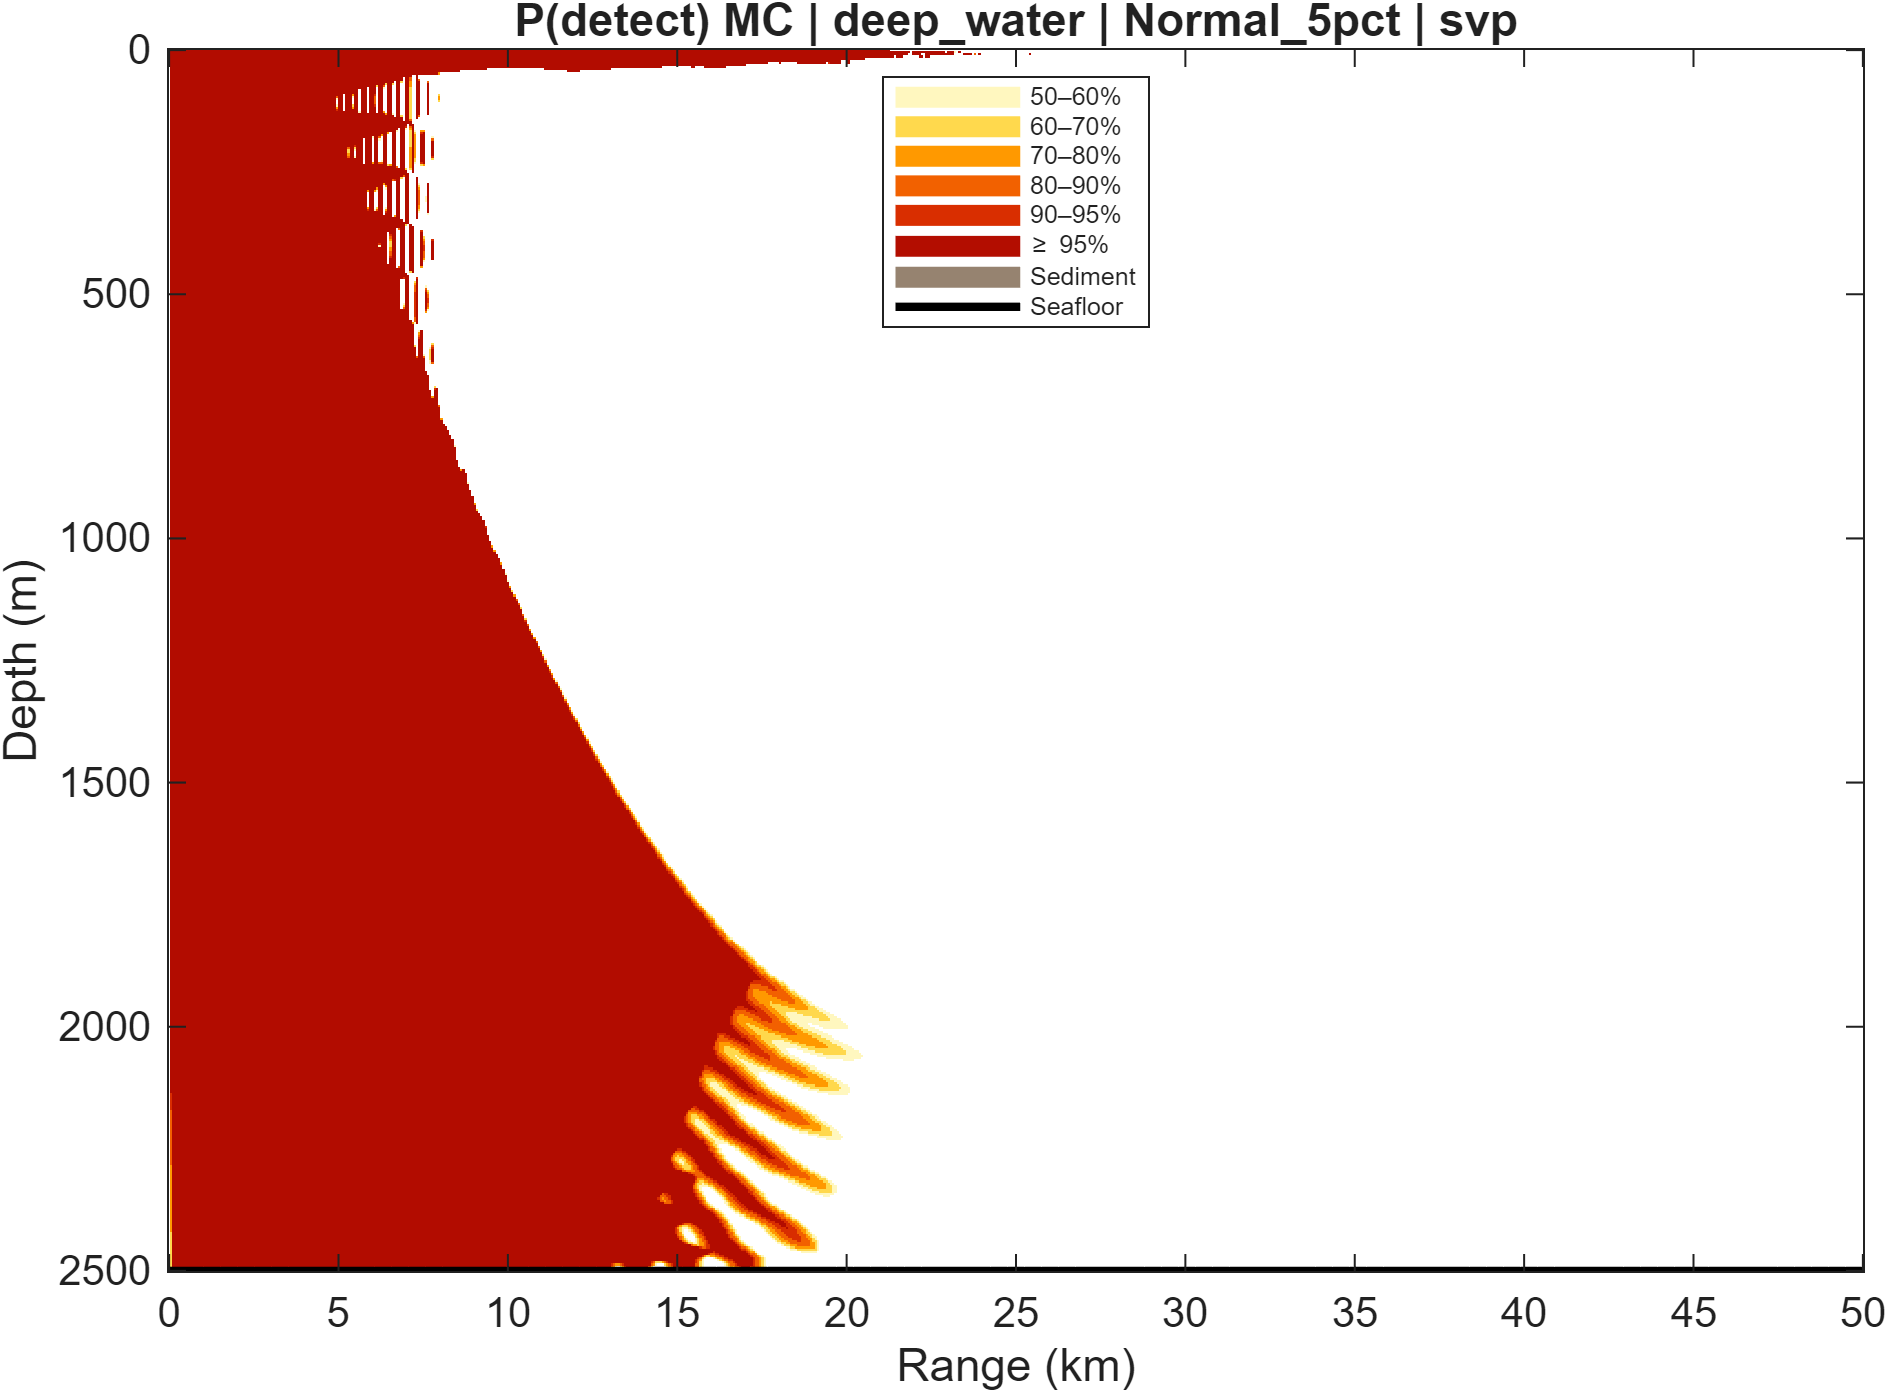
\includegraphics[width=\linewidth]{deep_water/Normal_5pct/figures/detect_empirical_svp.png}
    \caption{\small SVP}
  \end{subfigure}
\end{center}
$z_S$ (centre) produces the \textbf{largest shadow regions}, consistent with PCE non-convergence.
Variance alone does not reveal this asymmetry.
\end{block}

\vspace{0.5em}
\begin{block}{Method Recommendations}
\renewcommand{\arraystretch}{1.3}
\begin{center}
\begin{tabular}{p{3.5cm}ccc}\small
  \toprule
  \textbf{Scenario} & \textbf{1\%} & \textbf{5\%} & \textbf{10\%} \\
  \midrule
  Flat, freq/SVP
    & \textcolor{successgreen}{\textbf{Delta}}
    & \textcolor{warnyellow}{\textbf{PCE}}
    & \textcolor{warnyellow}{\textbf{PCE}} \\
  Flat, $z_S$
    & \textcolor{successgreen}{\textbf{Delta}}
    & \textcolor{failred}{\textbf{MC}}
    & \textcolor{failred}{\textbf{MC}} \\
  Slope
    & \textcolor{warnyellow}{\textbf{PCE}}
    & \textcolor{failred}{\textbf{MC}}
    & \textcolor{failred}{\textbf{MC}} \\
  \bottomrule
\end{tabular}
\end{center}
{\small \textcolor{successgreen}{$\bullet$}~Delta: 6 extra Bellhop runs, flat+small only.
\textcolor{warnyellow}{$\bullet$}~PCE: zero new runs, moderate nonlinearity.
\textcolor{failred}{$\bullet$}~MC: $N{=}1000$, always reliable.}
\end{block}

\vspace{0.5em}
\begin{block}{Key Conclusions}
\begin{enumerate}\small
  \item Bellhop-FD Jacobian validated: $L_1 < 5\%$ vs.\ closed-form waveguide.
  \item Bellhop-FD Delta: reliable only for flat geometry + $\leq1\%$ perturbation.
        2nd-order correction $>96\%$ of total variance at 5\% signals divergence.
  \item PCE converges for freq and SVP ($K^*{=}3$--6), zero new Bellhop runs.
  \item \textbf{$z_S$ in deep water resists PCE at all orders} --- SOFAR modal
        excitation nonlinearity; full MC required.
  \item LN3 practically useful ($D_\mathrm{KS} < 0.17$) despite formal rejection.
  \item Report $P_\mathrm{fail}$ and P95 --- not variance alone.
\end{enumerate}
\end{block}

\end{column}

\end{columns}

\end{frame}
\end{document}
